\section{Zihan's different Computational Experience}
\subsection{Brief}
In last winter semester,I started to learn R, Matlab and Stata. For Matlab and
Stata,I just konw some basic operation.For R, I learned some basic operations and also Monte Carlo models.
\subsection{experience}
 Mainly, the Monte Carlo model is used to generate simulated data and make predictions. In last
semester report, I used four regression models to predict GDP per capita and
then see which model has less error in predicting GDP per capita. Also, I
usd the regression models to calculate the estimated beta values and then see
which independent variables have a more significant effect on the dependent
variables.The result shows that LASSO performs the best by comparing the
effectiveness of four methods for predicting GDP per capita. 
\subsection{skills about latex}
\begin{align} 
    y2=x2+z2 \label{4}\\
    y3=x3+z3 \label{5}\\
    y3=x3+z3 \notag \\
    y4=x4+z4 \label{6}
\end{align}
$\sqrt{7}$, $\frac{1}{2}$.
\[ \pm\; \times \; \div\; \cdot\; \cap\; \cup\;\geq\; \leq\; \neq\; \approx \; \equiv \]
$ \sum_{i=1}^n i\quad \prod_{i=1}^n $  % \quad is a space equal to the current font size and \prod is a multiplication symbol
$ \sum\limits _{i=1}^n i\quad \prod\limits _{i=1}^n $ % \limits: compress these subscripts;\nolimits do not compress 
\[ \lim_{x\to0}x^2 \quad \int_a^b x^2 dx \]
\[ \lim\nolimits _{x\to0}x^2\quad \int\nolimits_a^b x^2 dx \]
\[ \iint\quad \iiint\quad \iiiint\quad \idotsint \]
\centering
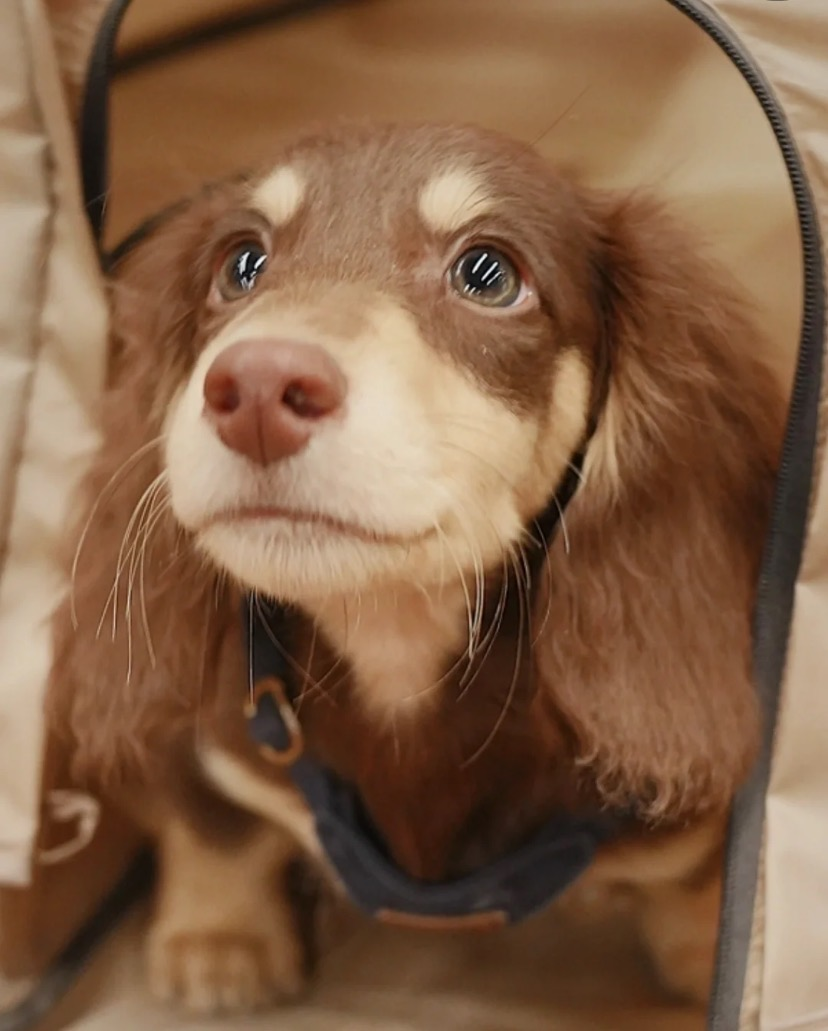
\includegraphics[width=0.7\textwidth]{dog.jpg}